De manière générale, un quadtree est une structure de données de type arbre dans laquelle chaque nœud possède quatre fils. Dans notre cas, on utilise un quadtree dit \enquote{région} qui représente l'image en deux dimensions, en décomposant la région en quatre parties égales, puis chaque partie en quatre sous-parties et ainsi de suite. Chaque nœud du quadtree représente un pixel noir, blanc ou gris. Un nœud gris contient un mélange de pixels blanc et noirs. On obtient un quadtree complet quand on subdivise l'image de manière récursive de manière à ce que le quadtree ne contienne que des nœuds de pixels blancs ou noirs.\\

Un quadtree \enquote{région} ayant une profondeur \texttt{n} peut être utilisé pour représenter une image de $2^{n}\times2^{n}$ pixels, où la valeur de chaque pixel est 0 (noir) ou 1 (blanc). Un exemple de quadtree est représenté dans la figure~\ref{fig:quadtree}.

\begin{figure}[H]
	\centering
	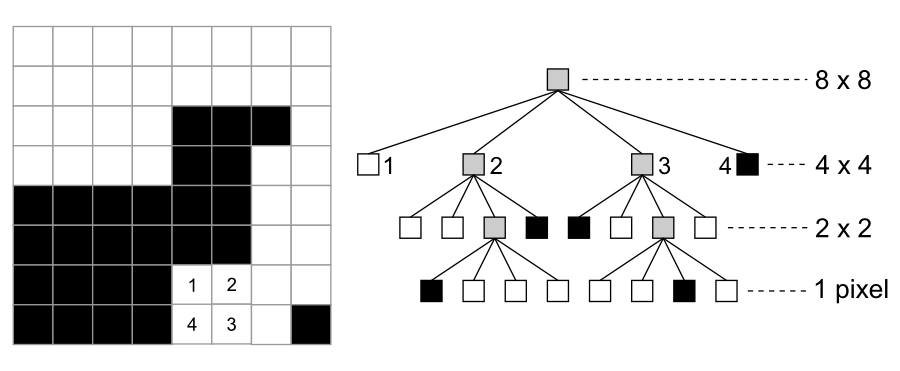
\includegraphics[scale=0.8]{images/quadTree.png}
	\caption{Représentation d'un quadtree}
	\label{fig:quadtree}
\end{figure}